\section{Particle Accelerators and CERN}

\subsection{Particle Accelerators}

%The first modern particle accelerators started to be conceived at the beginning of the 1900s. Those
%first accelerators, such as the Cockroft-Walton generator, used voltage multipliers to generate
%electric fields in order to accelerate particles.  Voltage multipliers are nowadays still an
%important piece of equipment as they are used in devices requiring high voltage, such as X-Ray
%machines, CRT monitors, microwaves or as part of an accelerator complex.  Those early technologies
%were namely used to perform the first artificial nuclear disintegration.

\todo{GPT}

The history of particle accelerators is a captivating narrative that spans over a century of
scientific innovation and discovery. It is a journey that has fundamentally transformed our
understanding of the universe's fundamental particles and their interactions. The concept of
accelerating particles to high speeds originated in the late 19th century, with early experiments
conducted by pioneers such as J.J. Thomson and Ernest Rutherford, who utilized basic devices like
cathode ray tubes to propel electrons.  One of the earliest breakthroughs in accelerator technology
was the Cockcroft-Walton accelerator, introduced in 1932 by John Cockcroft and Ernest Walton. This
pioneering device employed voltage multipliers to accelerate protons and ions, enabling the first
artificial nuclear disintegration—a milestone that earned them the Nobel Prize in Physics in 1951.
Building upon this achievement, the development of the synchrotron in the 1940s and 1950s by
scientists like Edwin McMillan and Vladimir Veksler marked a significant stride. Synchrotrons
harnessed magnetic fields to bend and accelerate charged particles in circular paths, advancing the
study of particle properties.  A key turning point emerged with the establishment of CERN (the
European Organization for Nuclear Research) in 1954, which culminated in the creation of the Proton
Synchrotron (PS) in 1959. This marked the emergence of a powerful era in accelerator science,
enabling the discovery of novel particles and laying the groundwork for the formulation of the
Standard Model of particle physics. Throughout the 1960s and 1970s, the advent of bubble chambers
and bubble chamber detectors provided researchers with the ability to trace the paths of charged
particles, leading to the revelation of various particles and their intricate interactions.  Yet,
the true marvel of accelerator technology came to the forefront with the construction of the Large
Hadron Collider (LHC) at CERN, which commenced operation in 2008. The LHC, an awe-inspiring
27-kilometer ring of superconducting magnets, propels protons and heavy ions to velocities nearing
the speed of light. The LHC's monumental achievement—the discovery of the Higgs boson in 2012—marked
a crowning moment in particle physics, solidifying the vital role of particle accelerators in
unraveling the fabric of the cosmos.  As particle physicists peer into the future, the quest
continues. Concepts such as linear colliders and advanced circular colliders are on the horizon,
promising to delve even deeper into the enigmatic realm of fundamental particles and the forces that
govern them. The history of particle accelerators underscores the profound human endeavor to explore
the most intricate mysteries of the universe, revealing the intricate dance of particles that shape
the cosmos and expanding the horizons of human knowledge.



\subsection{The CERN Complex}


\todo{GPT}
The CERN complex, located near Geneva, Switzerland, is a prominent center for particle physics
research. Its centerpiece is the Large Hadron Collider (LHC), the world's largest particle
accelerator with a 27-kilometer circumference. Here, protons and heavy ions are accelerated to near
light speed and collide at various points for fundamental particle studies. Surrounding the LHC are
significant particle detectors, including ATLAS, CMS, ALICE, and LHCb, designed to capture and
analyze particles generated during these collisions.  CERN also includes linear accelerators, the
Proton Synchrotron (PS), Super Proton Synchrotron (SPS), and Antiproton Decelerator (AD),
contributing to particle acceleration and antimatter research. Alongside these facilities, CERN
houses the Theoretical Physics Department, where theorists collaborate with experimentalists. With
research, administrative buildings, laboratories, and workshops, CERN provides a comprehensive
environment for scientific exploration. Its history, including the 2012 discovery of the Higgs
boson, underscores its importance in advancing particle physics and highlighting international
scientific cooperation.



%%%%%%%%%%%%%%%%%%%%%%%%%%%%%%%%%%%%%%%%%%%%%%%%%%%%%%%%%%%%%
%%%                       LHC
%%%%%%%%%%%%%%%%%%%%%%%%%%%%%%%%%%%%%%%%%%%%%%%%%%%%%%%%%%%%%
\subsection{The Large Hadron Collider}

\begin{figure}[H]
    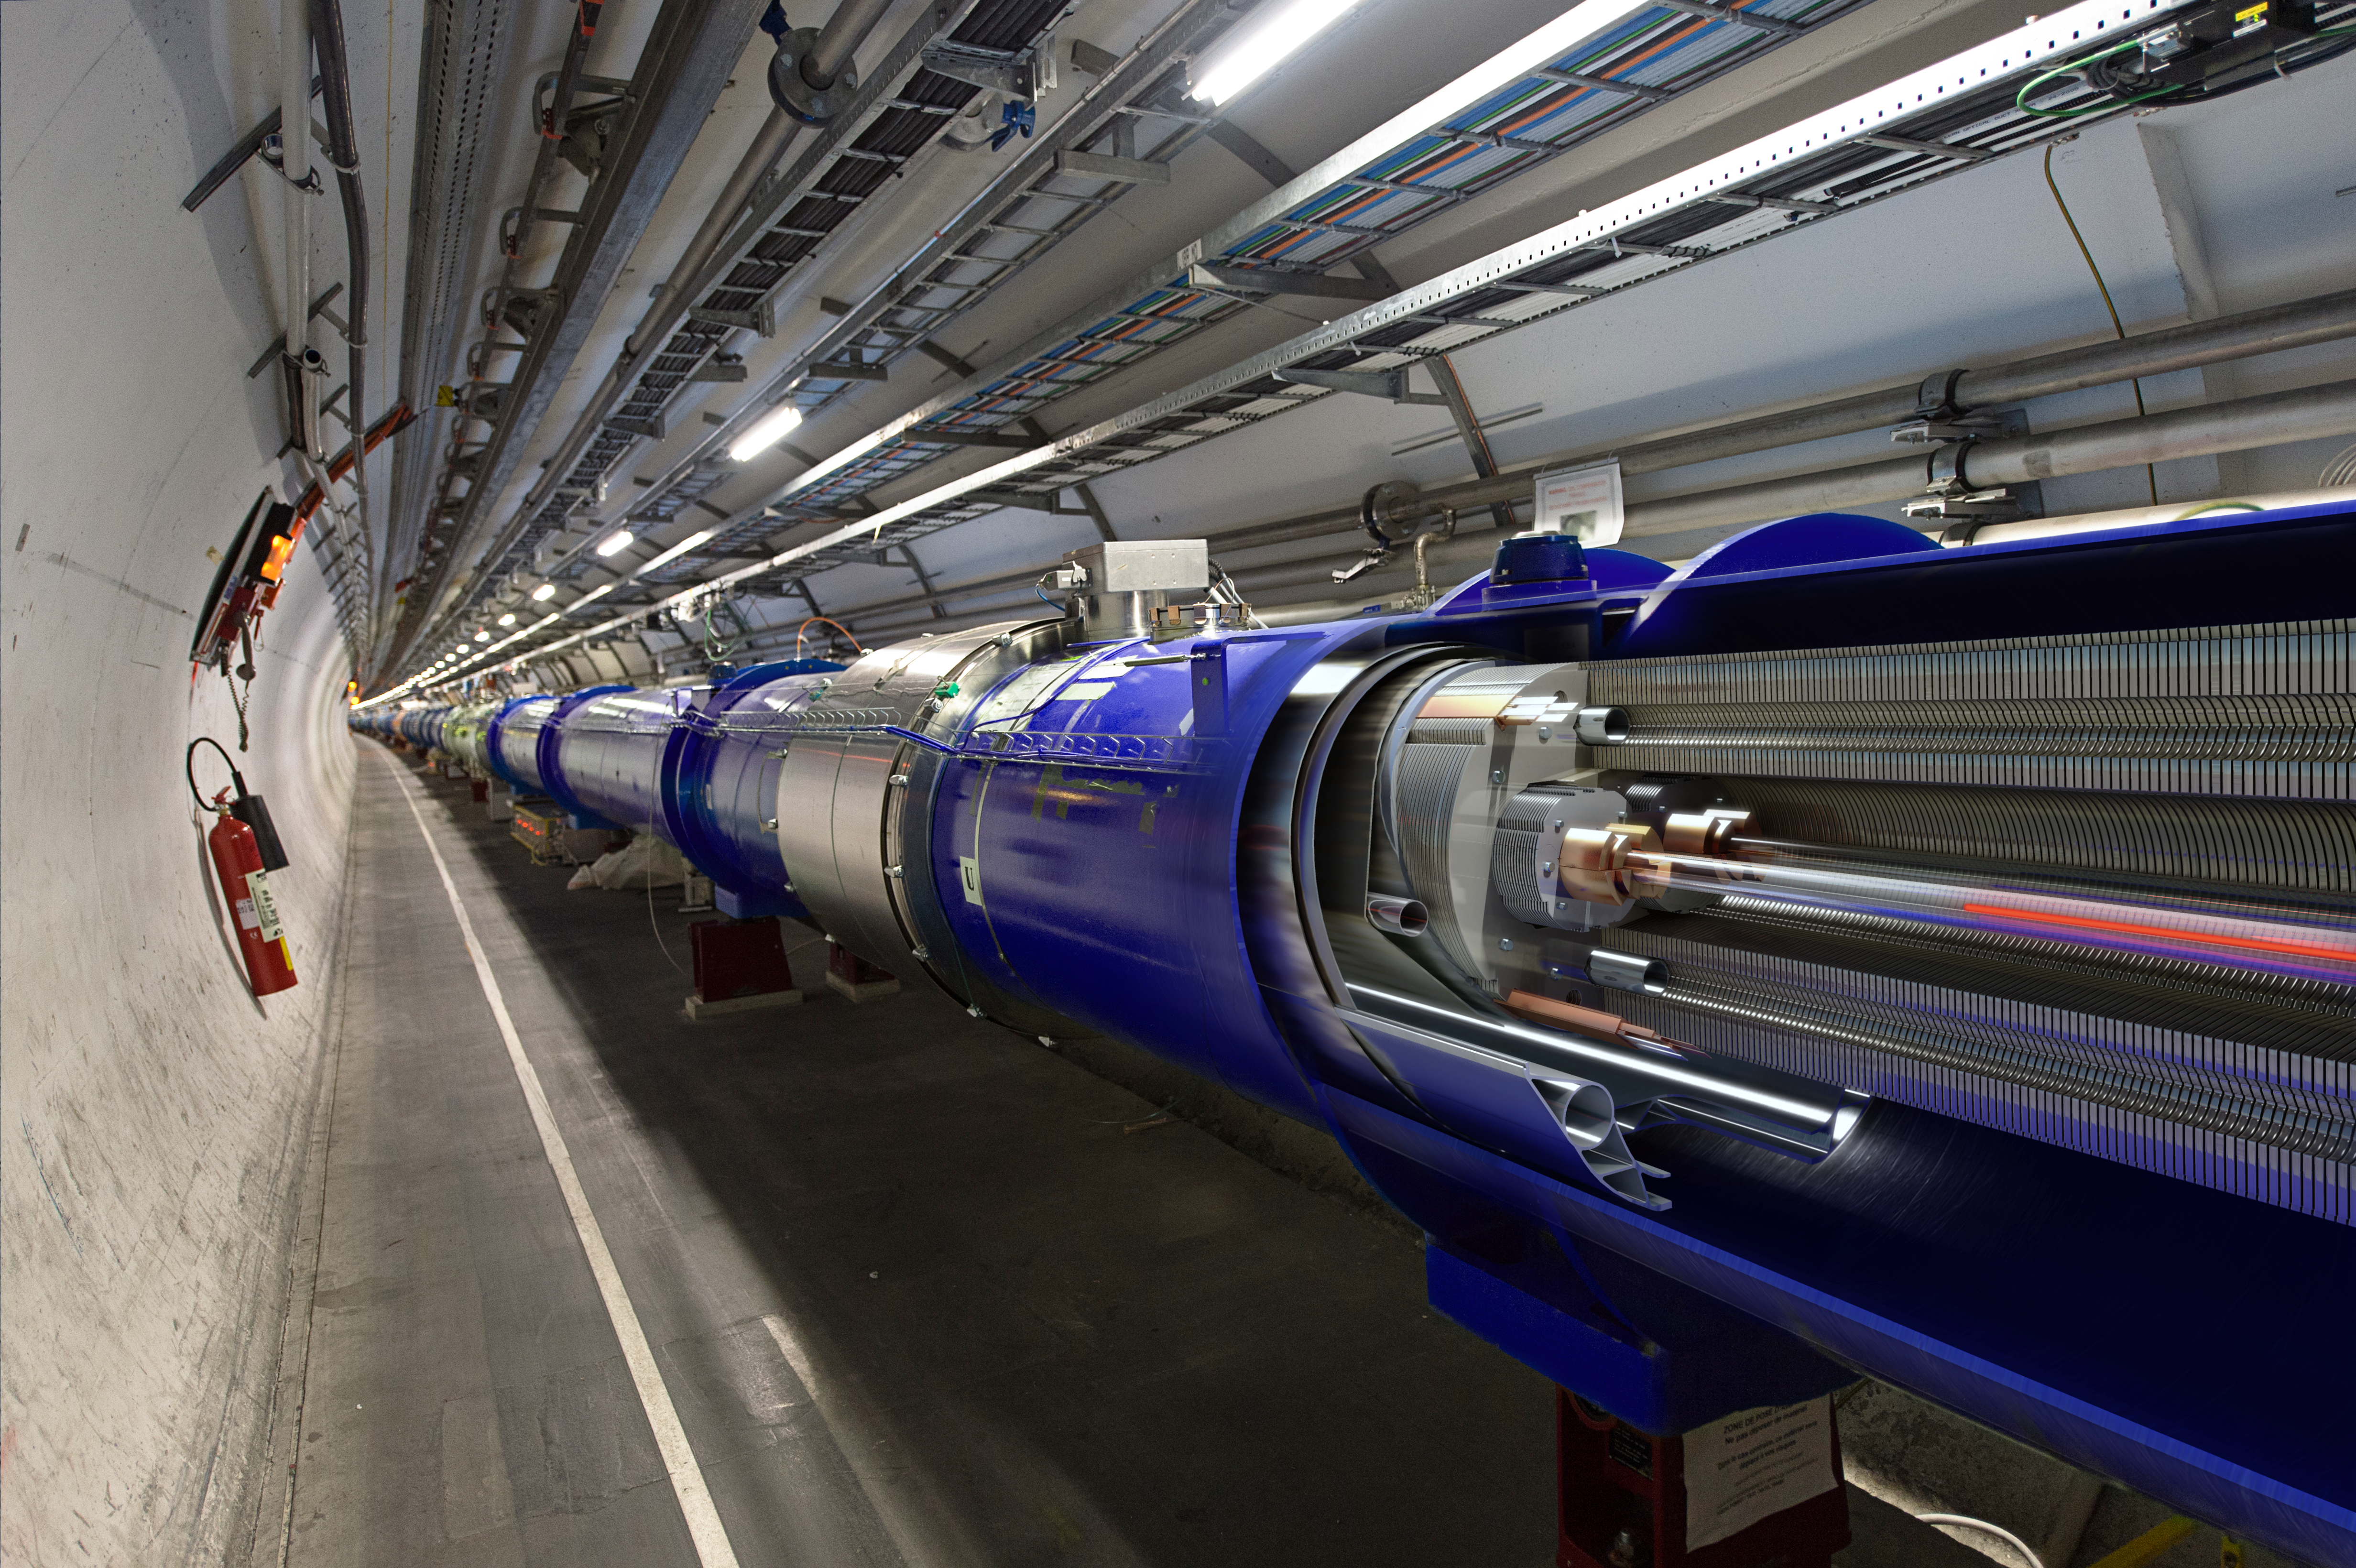
\includegraphics[width=\textwidth]{chapters/01_Introduction/images/lhc_3D_cut.png}
    \caption{3D cut of a main LHC dipole~\cite{noauthor_cern_nodate}.}
    \label{fig:3d_cut_dipole}
\end{figure}

speed of light, 11 000 turns per second, 12 000 amps in dipoles, number dipoles, price, parameters
energy consumption, detectors and experiments, discoveries, collimators, optics, magnets, luminosity, arcs, IRs, schematics, cryostat, beta function FODO

\begin{enumerate}
    \color{red}
    \item Cycles \& types of bunches: pilot for measurements
\end{enumerate}